\chapter{Design}\label{chap:design}

    Da wie bereits erwähnt, die Projekte \emph{"ITCS-Management"} und \emph{"ITCS"} bereits existierten, waren das grundlegende Design und sie technische Architektur bereits vorgegeben.
    Dies umfasst Aspekte wie die Transaktionsverwaltung der Datenbank als auch Elemente im Frontend wie die Navigation zwischen den Seiten oder die Farbpalette.

\section{"itcs-Management"}\label{sec:itcs-management-design}
    Im Projekt \emph{"itcs-Management"} wurde eine Vielzahl an kleineren Aufgaben erledigt. Dabei handelte es sich um Blazor-Seiten die meist nur Datenbank-Entitäten tabellarisch
    darstellen und beschränktes Editieren ermöglichen sollten. Im Bericht selbst wird auf diese Aufgaben, aufgrund ihrer repetitiven Natur nicht weiter eingegangen. Konzentriert wird sich 
    auf die größte Aufgabe in diesem Projekt namens \emph{"Umlaufeditor"}. 
    Ein Umlauf stellt dabei eine Sequenz von Fahrten dar, die von einem einzelnen Fahrzeug in einem Durchgang durchgeführt wird. Die Fahrten werden von den meisten Kunden in anderen 
    Systemen erstellt und sind mit dem Import neuer Versionen bereits in der Datenbank schon vorhanden. Die Umläufe hingegen werden nicht in anderen Systemen definiert und sollen deswegen
    mit diesem Editor erstellt und angepasst werden. 
    \begin{figure}[H]
        \centering
        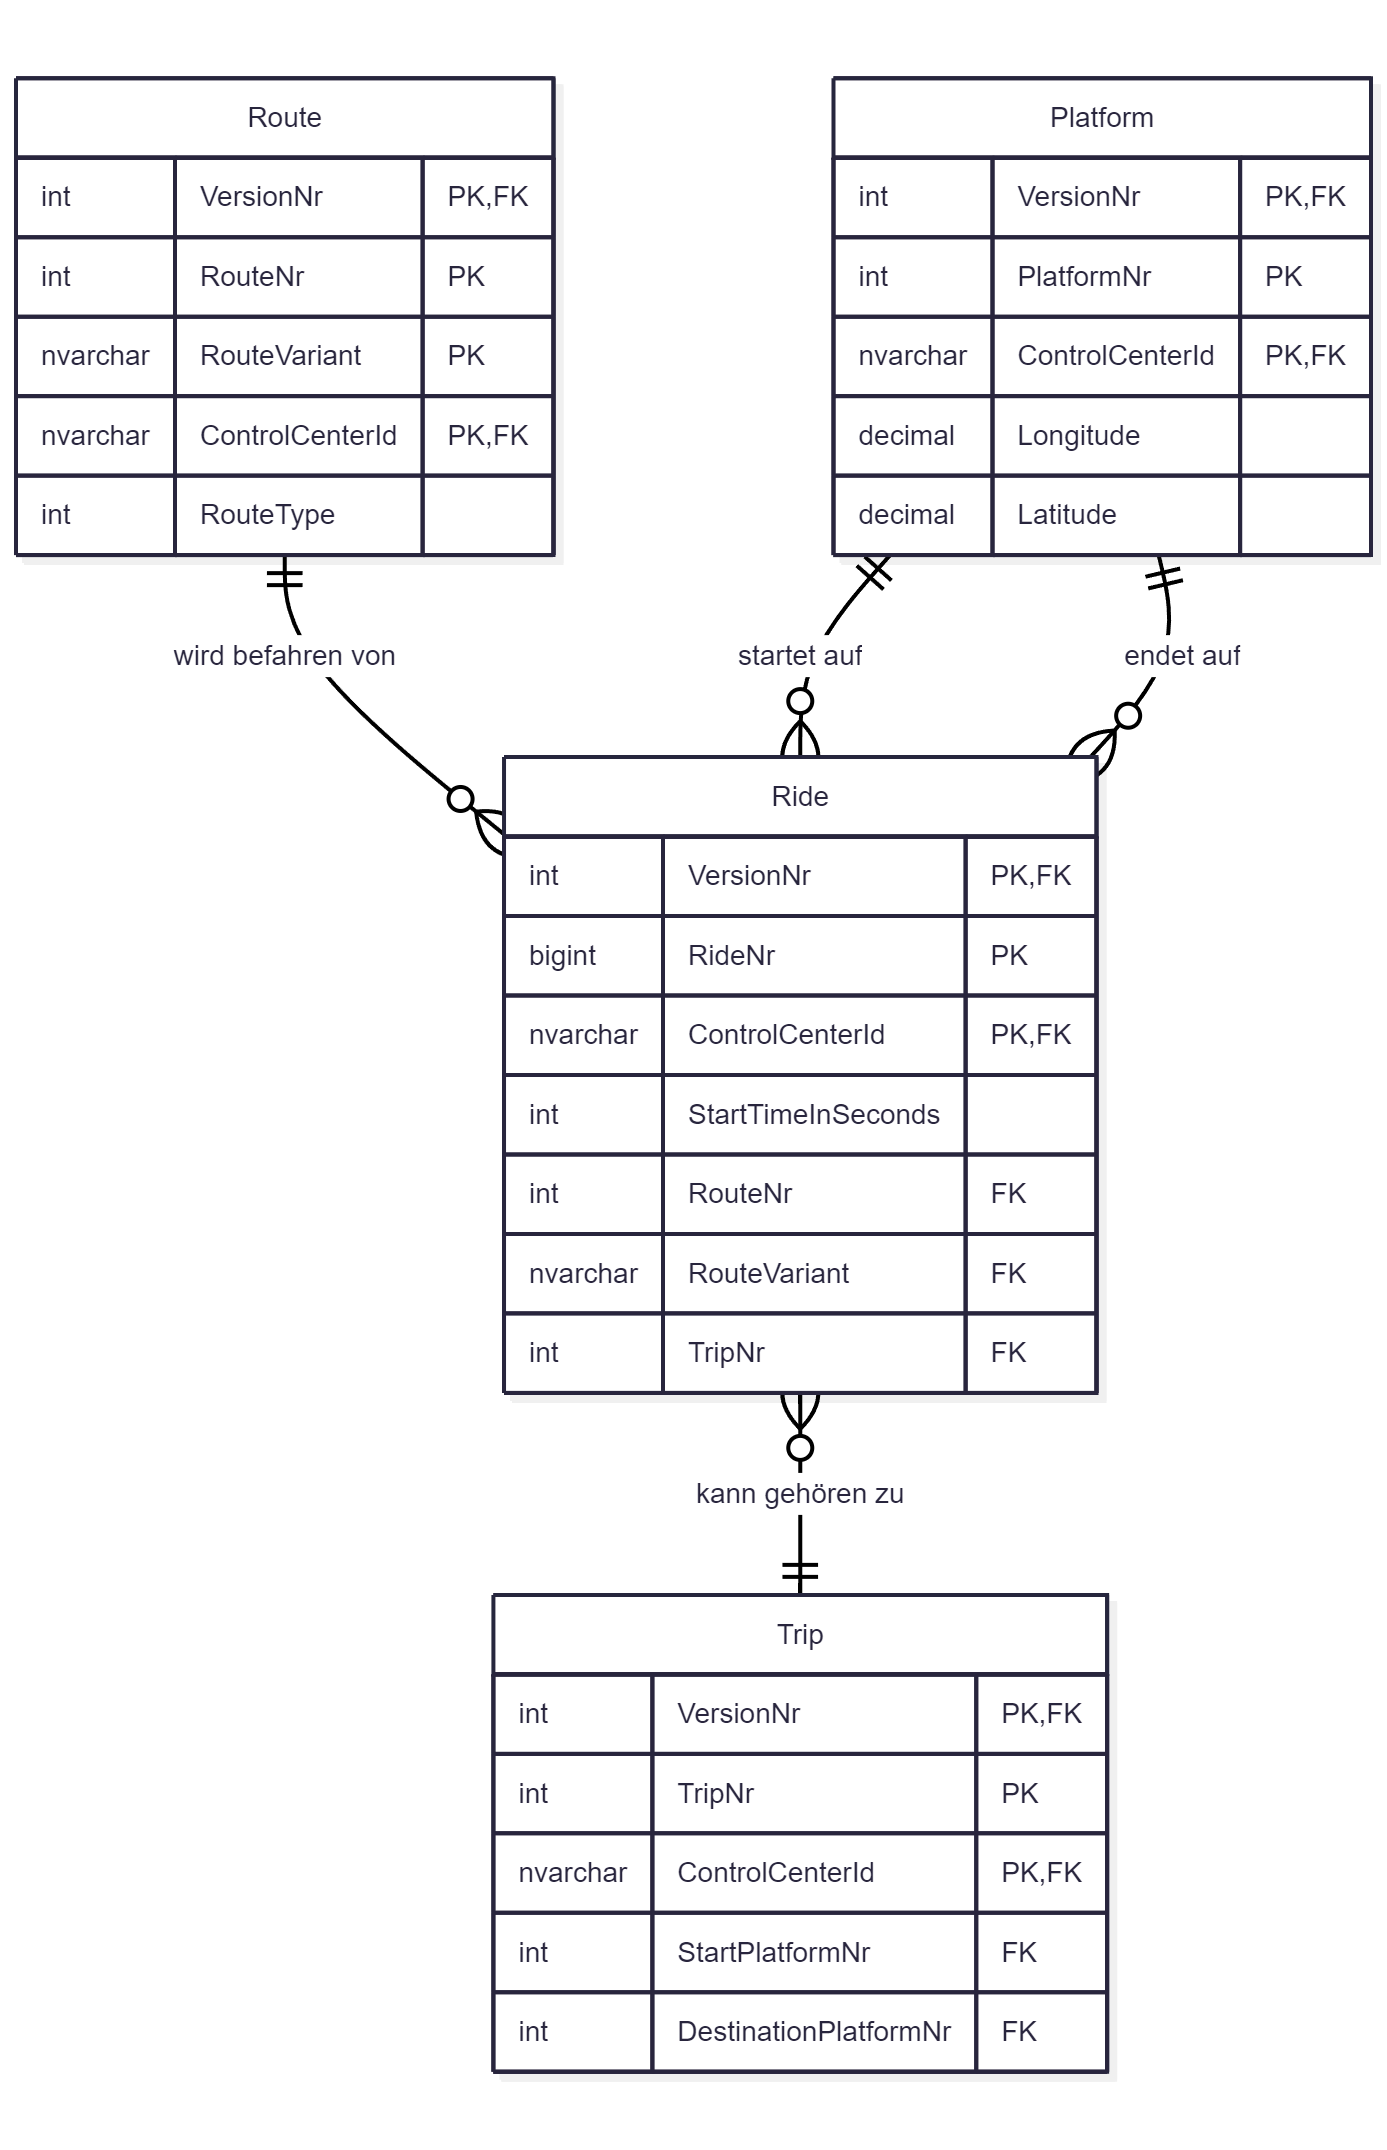
\includegraphics[width=0.8\textwidth]{transportation_system.png}
        \caption{Beziehungen von Umläufen und Fahrten}
        \label{fig:BeziehungenvonUmläufenundFahrten}
    \end{figure}

    Abbildung \ref{fig:BeziehungenvonUmläufenundFahrten} soll einen groben Überblick über das unmittelbar für diese Aufgabe benötigte Datenschema, verschaffen. Für das Verständnis unwesentliche 
    Datenkomponenten und Beziehungen wurden weglassen. Die Entität "Route" ist in diesem Modell deswegen wichtig, da die Datenkomponente "RouteNr" die Art der Fahrt festlegt. Für Pausen oder nicht produktiven
    Fahrten wird eine eigene Nummer vergeben. Zusätzlich ist bei jedem Umlauf ebenfalls jeweils eine Platform-Entität (auch "Steig") als Start- und Endpunkt eingetragen. Dabei kann es sich bei den 
    Steigen um Sonderhaltepunkte wie beispielsweise Betriebshöfen handeln.

    Der Umlaufeditor besteht aus folgenden 3 Blazor-Seiten: 
    \begin{itemize}
        \item \emph{Sonderhaltepunkte}: Da Sonderhaltepunkte von den meisten Kunden nicht mit externen Tools erstellt werden und somit nicht beim Import neuer Versionen inbegriffen sind, 
                erlaubt diese Seite die Verwaltung und Erstellung neuer Sonderhaltepunkte.
        \item \emph{Umläufen}: Diese Seite stellt das Herzstück des Umlaufeditors dar. Hier können neue Umläufe erstellt und mit Fahrten versehen werden. Außerdem können bestehende Umläufe 
                als Vorlagen abgespeichert werden. 
        \item \emph{Vorlagen}: Hier können alle bestehenden Vorlagen eingesehen werden. Sollten für einen Umlauf mehrere Vorlagen bestehen oder Vorlagen in Zukunft nicht mehr durchführbar sein, können diese
                deaktiviert oder gelöscht werden.
    \end{itemize}

    % \begin{figure}[H]
    %     \centering
    %     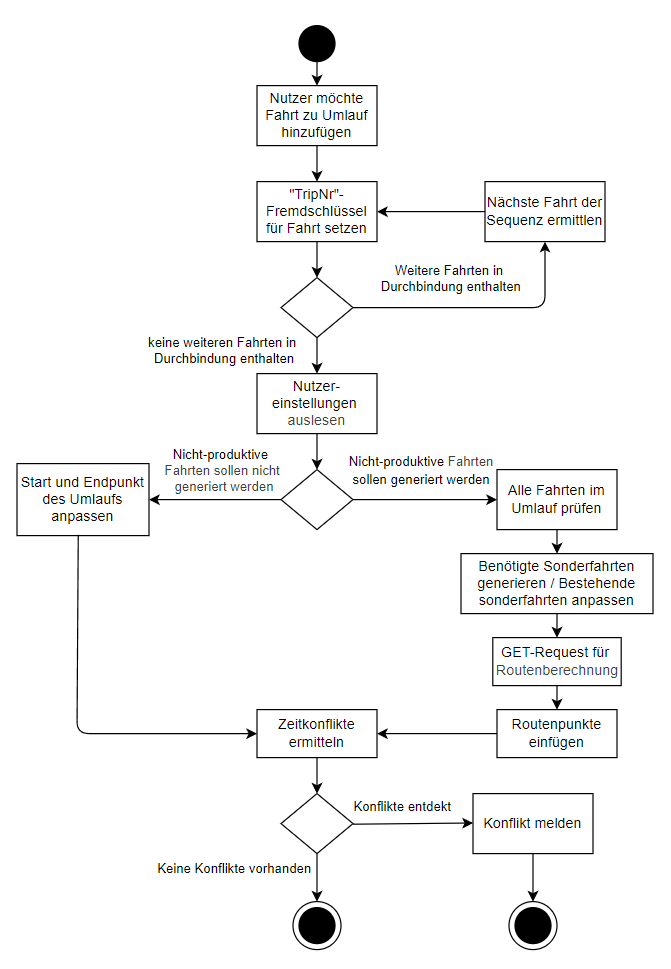
\includegraphics[width=0.8\textwidth]{Ablauf.png}
    %     \caption{Beziehungen von Umläufen und Fahrten}
    %     \label{fig:Ablauf}
    % \end{figure}


